% SC3099 --- Chapter 4: Project Planning: Agile, Risk, and Scheduling (0->100 ground-up)
\chapter{Project Planning: Agile, Risk, and Scheduling}
\label{ch:planning}

\begin{quote}
\emph{``Plans are worthless, but planning is everything.''} --- Eisenhower. A capstone fails not from lack of code but from lack of coordination. This chapter turns vague ambition into a scheduled, risk-aware sprint plan you can execute and defend.
\end{quote}

\noindent\fbox{\parbox{\dimexpr\linewidth-2\fboxsep-2\fboxrule}{%
\textbf{From zero: no project-management background assumed.} We define \emph{sprint}, \emph{backlog}, \emph{risk}, \emph{Gantt}, and \emph{estimation} from scratch---intuition and pictures before formalism. No prior Agile or scheduling knowledge is assumed. We build on proposal (Ch.~1), requirements (Ch.~2), and design (Ch.~3).}}
\vspace{0.4em}

\section*{Learning Outcomes}
After this chapter you will be able to:
\begin{enumerate}[label=(L\arabic*)]
    \item run Scrum sprints for a capstone: roles, backlog, sprint planning, stand-ups, review, and retrospective;
    \item identify, assess, and mitigate project risks using a likelihood$\times$impact matrix and a risk register;
    \item construct and read a Gantt chart, identify the critical path, and reason about dependencies and slack;
    \item estimate work with story points and planning poker and translate estimates into a sprint capacity plan;
    \item detect planning smells (over-commitment, invisible risk, waterfall-in-scrum) and correct them early.
\end{enumerate}

% ============================================================
\section{Agile for Capstone: Scrum Sprints, Backlog, and Stand-ups}
\label{sec:agile-capstone}
Waterfall pretends requirements are frozen; capstone reality is iterative---supervisor feedback, API limits, and integration surprises change scope weekly. \emph{Agile} embraces change by delivering in short, fixed-length \emph{sprints} (1--2 weeks) that each produce a demoable increment.

\paragraph{Scrum in miniature.} Three roles: \emph{Product Owner} (owns priority---often the team jointly with supervisor), \emph{Scrum Master} (protects process), \emph{Developers} (build). One \emph{product backlog} (ordered list of user stories/features). Each sprint: \emph{sprint planning} (pick top items you can finish), \emph{daily stand-up} (15 min: what I did / will do / blocker), \emph{sprint review} (demo to stakeholders), \emph{retrospective} (what to improve). For a 4-person FYP, combine roles pragmatically but keep the ceremonies.

\paragraph{Backlog and Kanban.} A user story: ``As a \emph{role} I want \emph{goal} so that \emph{value}.'' Add acceptance criteria and a size estimate. The \emph{sprint board} makes work visible: columns \texttt{To Do} $\to$ \texttt{Doing} $\to$ \texttt{Done}; WIP limits prevent starting everything and finishing nothing.

\begin{figure}[h]
\centering
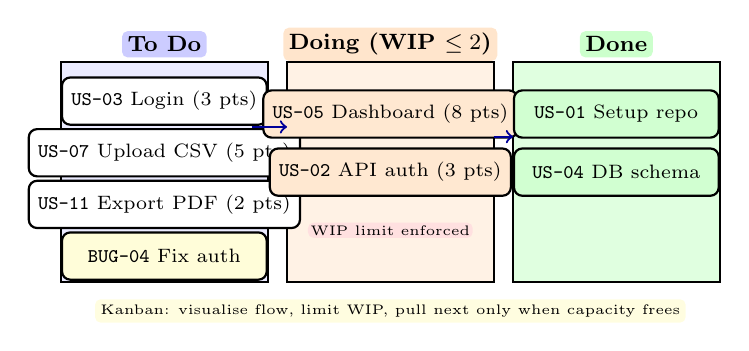
\begin{tikzpicture}[scale=0.82, every node/.style={font=\scriptsize}]
% columns
\fill[blue!8] (0,0) rectangle (3.2,-3.4);
\fill[orange!10] (3.5,0) rectangle (6.7,-3.4);
\fill[green!12] (7.0,0) rectangle (10.2,-3.4);
\draw[thick] (0,0) rectangle (3.2,-3.4);
\draw[thick] (3.5,0) rectangle (6.7,-3.4);
\draw[thick] (7.0,0) rectangle (10.2,-3.4);
\node[font=\footnotesize\bfseries,fill=blue!20,rounded corners=2pt,inner sep=2pt] at (1.6,0.28) {To Do};
\node[font=\footnotesize\bfseries,fill=orange!20,rounded corners=2pt,inner sep=2pt] at (5.1,0.28) {Doing (WIP $\le 2$)};
\node[font=\footnotesize\bfseries,fill=green!20,rounded corners=2pt,inner sep=2pt] at (8.6,0.28) {Done};
% cards ToDo
\node[draw,thick,fill=white,rounded corners=3pt,minimum width=2.6cm,minimum height=0.6cm] at (1.6,-0.6) {\texttt{US-03} Login (3 pts)};
\node[draw,thick,fill=white,rounded corners=3pt,minimum width=2.6cm,minimum height=0.6cm] at (1.6,-1.4) {\texttt{US-07} Upload CSV (5 pts)};
\node[draw,thick,fill=white,rounded corners=3pt,minimum width=2.6cm,minimum height=0.6cm] at (1.6,-2.2) {\texttt{US-11} Export PDF (2 pts)};
\node[draw,thick,fill=yellow!15,rounded corners=3pt,minimum width=2.6cm,minimum height=0.6cm] at (1.6,-3.0) {\texttt{BUG-04} Fix auth};
% Doing
\node[draw,thick,fill=orange!18,rounded corners=3pt,minimum width=2.6cm,minimum height=0.6cm] at (5.1,-0.8) {\texttt{US-05} Dashboard (8 pts)};
\node[draw,thick,fill=orange!18,rounded corners=3pt,minimum width=2.6cm,minimum height=0.6cm] at (5.1,-1.7) {\texttt{US-02} API auth (3 pts)};
\node[font=\tiny,fill=red!12,rounded corners=2pt,inner sep=1pt] at (5.1,-2.6) {WIP limit enforced};
% Done
\node[draw,thick,fill=green!18,rounded corners=3pt,minimum width=2.6cm,minimum height=0.6cm] at (8.6,-0.8) {\texttt{US-01} Setup repo \checkmark};
\node[draw,thick,fill=green!18,rounded corners=3pt,minimum width=2.6cm,minimum height=0.6cm] at (8.6,-1.7) {\texttt{US-04} DB schema \checkmark};
\draw[->,thick,blue!60!black] (2.95,-1.0) -- (3.5,-1.0);
\draw[->,thick,blue!60!black] (6.7,-1.15) -- (7.0,-1.15);
\node[font=\tiny,align=center,fill=yellow!12,rounded corners=2pt,inner sep=2pt] at (5.1,-3.85) {Kanban: visualise flow, limit WIP, pull next only when capacity frees};
\end{tikzpicture}
\caption{Sprint board (Kanban): stories flow To Do $\to$ Doing $\to$ Done. WIP limit in Doing prevents thrashing; Done requires meeting Definition of Done (tested, reviewed, demoable).}
\label{fig:sprint-board}
\end{figure}

\paragraph{Definition of Done (DoD).} A story is not done when code is written but when it is \emph{tested, reviewed, documented, and demoable}. Agree a DoD checklist and enforce it at review---otherwise ``almost done'' piles up silently.

\begin{lstlisting}[language=Python, caption={Sprint backlog as code: machine-readable, filterable, and auditable.}]
# sprint_backlog.py -- single source of truth for sprint 2
sprint_backlog = [
    {"id": "US-03", "title": "User login", "pts": 3, "status": "ToDo",
     "acceptance": ["JWT issued", "401 on bad pw"], "owner": "Asha"},
    {"id": "US-05", "title": "Dashboard chart", "pts": 8, "status": "Doing",
     "acceptance": ["renders <1s for 10k rows"], "owner": "Ben"},
    {"id": "US-02", "title": "API auth middleware", "pts": 3, "status": "Doing",
     "owner": "Chen"},
    {"id": "BUG-04", "title": "Fix token refresh", "pts": 2, "status": "ToDo",
     "owner": "Dana"},
]
# capacity check: sum pts in sprint <= velocity (e.g., 14 pts/sprint)
velocity = 14
load = sum(s["pts"] for s in sprint_backlog if s["status"] != "Done")
print(f"Sprint load {load} / velocity {velocity} -> {'OK' if load <= velocity else 'OVER'}")
\end{lstlisting}

\section{Risk Management: Identify, Assess, Mitigate}
\label{sec:risk}
A \emph{risk} is an uncertain event that, if it occurs, affects objectives. Manage it in three steps: \emph{identify} (list it), \emph{assess} (likelihood $\times$ impact), \emph{mitigate} (reduce likelihood or impact, or have a contingency).

\paragraph{Risk register.} A table with columns: ID, description, cause, likelihood (L/M/H), impact (L/M/H), exposure, owner, mitigation, contingency, trigger. Review it every sprint---new risks appear as you integrate.

\begin{figure}[h]
\centering
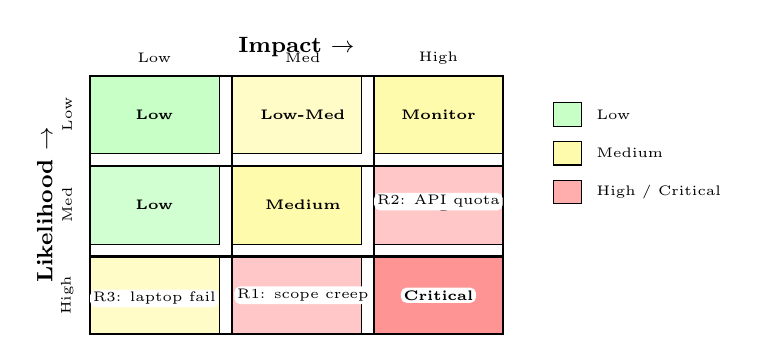
\begin{tikzpicture}[scale=0.82, every node/.style={font=\scriptsize}]
% grid 3x3 with heatmap
\foreach \x/\col in {0/green!18, 2.2/yellow!22, 4.4/red!18} {
  \foreach \y in {0,1.4,2.8} {
    \fill[\col] (\x,-\y) rectangle (\x+2.0,-\y-1.2);
    \draw[thick] (\x,-\y) rectangle (\x+2.0,-\y-1.2);
  }
}
% override to make proper heatmap: likelihood rows bottom->top, impact cols left->right
% Correct colors per cell (Low likelihood bottom row, High top)
\fill[green!22] (0,0) rectangle (2.0,-1.2);      % Low L, Low I
\fill[yellow!22] (2.2,0) rectangle (4.2,-1.2);   % Low L, Med I
\fill[yellow!32] (4.4,0) rectangle (6.4,-1.2);   % Low L, High I
\fill[green!18] (0,-1.4) rectangle (2.0,-2.6);   % Med L, Low I
\fill[yellow!32] (2.2,-1.4) rectangle (4.2,-2.6);% Med L, Med I
\fill[red!22] (4.4,-1.4) rectangle (6.4,-2.6);   % Med L, High I
\fill[yellow!22] (0,-2.8) rectangle (2.0,-4.0);  % High L, Low I
\fill[red!22] (2.2,-2.8) rectangle (4.2,-4.0);   % High L, Med I
\fill[red!42] (4.4,-2.8) rectangle (6.4,-4.0);   % High L, High I
\draw[thick] (0,0) rectangle (6.4,-4.0);
\draw[thick] (2.2,0) -- (2.2,-4.0); \draw[thick] (4.4,0) -- (4.4,-4.0);
\draw[thick] (0,-1.4) -- (6.4,-1.4); \draw[thick] (0,-2.8) -- (6.4,-2.8);
% labels
\node[font=\tiny\bfseries] at (1.0,-0.6) {Low};
\node[font=\tiny\bfseries] at (3.3,-0.6) {Low-Med};
\node[font=\tiny\bfseries] at (5.4,-0.6) {Monitor};
\node[font=\tiny\bfseries] at (1.0,-2.0) {Low};
\node[font=\tiny\bfseries] at (3.3,-2.0) {Medium};
\node[font=\tiny\bfseries] at (5.4,-2.0) {High};
\node[font=\tiny\bfseries] at (1.0,-3.4) {Medium};
\node[font=\tiny\bfseries] at (3.3,-3.4) {High};
\node[font=\tiny\bfseries,fill=white,rounded corners=2pt,inner sep=1pt] at (5.4,-3.4) {Critical};
% example risks placed
\node[font=\tiny,fill=white,rounded corners=2pt,inner sep=1pt] at (5.4,-1.95) {R2: API quota};
\node[font=\tiny,fill=white,rounded corners=2pt,inner sep=1pt] at (3.3,-3.4) {R1: scope creep};
\node[font=\tiny,fill=white,rounded corners=2pt,inner sep=1pt] at (1.0,-3.45) {R3: laptop fail};
% axes
\node[font=\footnotesize\bfseries] at (3.2,0.45) {Impact $\rightarrow$};
\node[font=\footnotesize\bfseries,rotate=90] at (-0.7,-2.0) {Likelihood $\rightarrow$};
\node[font=\tiny] at (1.0,0.28) {Low}; \node[font=\tiny] at (3.3,0.28) {Med}; \node[font=\tiny] at (5.4,0.28) {High};
\node[font=\tiny,rotate=90] at (-0.35,-0.6) {Low}; \node[font=\tiny,rotate=90] at (-0.35,-2.0) {Med}; \node[font=\tiny,rotate=90] at (-0.35,-3.4) {High};
% legend
\node[draw,fill=green!22,minimum width=0.35cm,minimum height=0.3cm] at (7.4,-0.6) {};
\node[font=\tiny,anchor=west] at (7.7,-0.6) {Low};
\node[draw,fill=yellow!32,minimum width=0.35cm,minimum height=0.3cm] at (7.4,-1.2) {};
\node[font=\tiny,anchor=west] at (7.7,-1.2) {Medium};
\node[draw,fill=red!32,minimum width=0.35cm,minimum height=0.3cm] at (7.4,-1.8) {};
\node[font=\tiny,anchor=west] at (7.7,-1.8) {High / Critical};
\end{tikzpicture}
\caption{Risk matrix: likelihood $\times$ impact heatmap. Green = accept/monitor, yellow = mitigate, red = active mitigation + contingency. Example risks plotted: scope creep, API quota, hardware failure.}
\label{fig:risk-matrix}
\end{figure}

Example entries: \texttt{R1} Scope creep (M likelihood, H impact) $\to$ mitigate by freezing sprint scope, contingency: descope stretch goals. \texttt{R2} Third-party API rate limit (M/H) $\to$ cache + mock, fallback dataset. \texttt{R3} Hardware loss (L/M) $\to$ daily push to Git, cloud backup. Assign an \emph{owner} per risk---unowned risks are unmanaged.

\section{Gantt and Scheduling: From Dependencies to Critical Path}
\label{sec:gantt}
A \emph{Gantt chart} maps tasks to calendar time as horizontal bars; arrows show dependencies. It answers ``what must finish before what can start?'' and ``where is the \emph{critical path}---the longest chain with zero slack?'' Delay on the critical path delays the project; delay off it may be absorbed.

\begin{figure}[h]
\centering
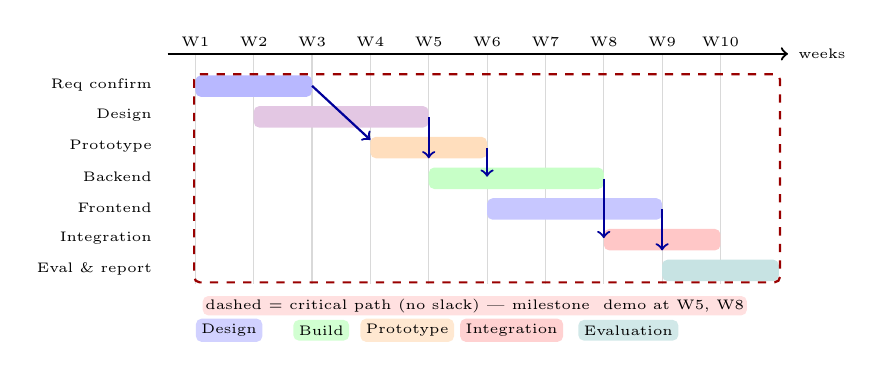
\begin{tikzpicture}[scale=0.78, every node/.style={font=\scriptsize}]
% grid weeks 1..10
\foreach \w in {1,...,10} {
  \node[font=\tiny] at (\w*0.95,0.35) {W\w};
  \draw[gray!30] (\w*0.95,0.15) -- (\w*0.95,-3.6);
}
\draw[thick,->] (0.5,0.15) -- (10.6,0.15) node[right,font=\tiny] {weeks};
% task labels
\node[font=\tiny,anchor=east] at (0.4,-0.35) {Req confirm};
\node[font=\tiny,anchor=east] at (0.4,-0.85) {Design};
\node[font=\tiny,anchor=east] at (0.4,-1.35) {Prototype};
\node[font=\tiny,anchor=east] at (0.4,-1.85) {Backend};
\node[font=\tiny,anchor=east] at (0.4,-2.35) {Frontend};
\node[font=\tiny,anchor=east] at (0.4,-2.85) {Integration};
\node[font=\tiny,anchor=east] at (0.4,-3.35) {Eval \& report};
% bars (x = week start, width = duration)
\fill[blue!28,rounded corners=2pt] (0.95,-0.55) rectangle (2.85,-0.20);   % W1-2
\fill[violet!22,rounded corners=2pt] (1.90,-1.05) rectangle (4.75,-0.70); % W2-4
\fill[orange!26,rounded corners=2pt] (3.80,-1.55) rectangle (5.70,-1.20); % W4-5
\fill[green!22,rounded corners=2pt] (4.75,-2.05) rectangle (7.60,-1.70);  % W5-7
\fill[blue!22,rounded corners=2pt] (5.70,-2.55) rectangle (8.55,-2.20);   % W6-8
\fill[red!22,rounded corners=2pt] (7.60,-3.05) rectangle (9.50,-2.70);    % W8-9
\fill[teal!22,rounded corners=2pt] (8.55,-3.55) rectangle (10.45,-3.20);  % W9-10
% dependencies arrows
\draw[->,thick,blue!60!black] (2.85,-0.37) -- (3.80,-1.25);
\draw[->,thick,blue!60!black] (4.75,-0.88) -- (4.75,-1.55);
\draw[->,thick,blue!60!black] (5.70,-1.38) -- (5.70,-1.85);
\draw[->,thick,blue!60!black] (7.60,-1.88) -- (7.60,-2.85);
\draw[->,thick,blue!60!black] (8.55,-2.38) -- (8.55,-3.05);
% critical path highlight (top border)
\draw[thick,red!60!black,dashed,rounded corners=2pt] (0.93,-0.18) rectangle (10.47,-3.57);
\node[font=\tiny,fill=red!12,rounded corners=2pt,inner sep=1pt] at (5.5,-3.95) {dashed = critical path (no slack) --- milestone $\blacktriangleright$ demo at W5, W8};
% legend
\node[font=\tiny,fill=blue!18,rounded corners=2pt,inner sep=2pt] at (1.5,-4.35) {Design};
\node[font=\tiny,fill=green!18,rounded corners=2pt,inner sep=2pt] at (3.0,-4.35) {Build};
\node[font=\tiny,fill=orange!18,rounded corners=2pt,inner sep=2pt] at (4.4,-4.35) {Prototype};
\node[font=\tiny,fill=red!18,rounded corners=2pt,inner sep=2pt] at (6.1,-4.35) {Integration};
\node[font=\tiny,fill=teal!18,rounded corners=2pt,inner sep=2pt] at (8.0,-4.35) {Evaluation};
\end{tikzpicture}
\caption{Gantt chart for a 10-week capstone slice: bars = tasks, arrows = dependencies, dashed envelope = critical path. Parallel tracks (Backend/Frontend) show where slack exists.}
\label{fig:gantt}
\end{figure}

Keep the Gantt \emph{living}: update actuals weekly, mark milestones ($\blacktriangleright$ demos, submission), and re-plan when estimates drift. A stale Gantt is worse than none---it gives false confidence.

\section{Estimation: Story Points and Planning Poker}
\label{sec:estimation}
Estimating in hours is noisy (``how many hours is login?''). \emph{Story points} estimate \emph{relative effort} on a Fibonacci scale (1,2,3,5,8,13): a 5 is roughly twice a 3, not ``5 hours.'' Velocity (points completed per sprint) is measured empirically and used to forecast.

\paragraph{Planning poker.} Each estimator privately picks a card (1--13), reveals simultaneously, then discusses outliers. This counters anchoring (first speaker bias) and surfaces hidden assumptions (``you assumed OAuth is ready; it is not''). Re-estimate until convergence within one step.

\paragraph{From points to schedule.} After 2--3 sprints you know velocity $v$ (e.g., 14 pts/sprint). Remaining backlog $B$ points $\to$ $\lceil B/v\rceil$ sprints required. If $\lceil B/v\rceil$ exceeds sprints left, descope now---not in week 12. Track a \emph{burn-down chart} (remaining points vs.\ sprint) to make slippage visible early.

\begin{remark}[Planning smells to watch]
Over-commitment (load $>$ velocity every sprint), invisible risk (no red cells owned), waterfall-in-scrum (Gantt with no parallel tracks or reviews), and point inflation (everything is 13) all signal a plan that looks good on paper but will slip.
\end{remark}

\section{Chapter Notes}
Scrum Guide (Schwaber \& Sutherland) defines the minimal Scrum; capstone adaptations are discussed in Fox \& Patterson, \emph{Engineering Software as a Service}. Risk heatmaps follow ISO~31000; Gantt (1910s) remains the clearest dependency visual when kept to 10--15 tasks. Planning poker is Grenning (2002); story-point forecasting is Cohn, \emph{Agile Estimation}.

\section{Exercises}
\label{sec:ch04-exercises}
\begin{enumerate}[label=E4.\arabic*, leftmargin=*, itemsep=0.8em]
    \item \textbf{Kanban flow.} Your Doing column has 4 cards, each blocked on code review. Using Fig.~\ref{fig:sprint-board} and WIP limits, explain why starting a 5th card hurts throughput. Propose a WIP policy and a stand-up rule to unblock flow.
    \item \textbf{Risk register.} Identify 5 capstone risks (technical, schedule, stakeholder, dependency, data/privacy). Place each on Fig.~\ref{fig:risk-matrix}, assign L/M/H, and for the two red cells write mitigation + contingency + trigger.
    \item \textbf{Gantt critical path.} From Fig.~\ref{fig:gantt}, list the task chain with zero slack. If Backend slips by 1 week, which downstream tasks and milestones move? If Frontend slips by 1 week but Backend does not, does the final deadline move? Why?
    \item \textbf{Planning poker estimation.} Stories: A=login, B=dashboard chart (10k rows), C=CSV import with validation. As a team, assign Fibonacci points using planning poker. Justify why B $>$ A and where C's uncertainty lies. After sprint 1 velocity = 12, backlog = 48 pts---how many sprints needed and what do you descope if only 3 sprints remain?
    \item \textbf{Sprint plan as code.} Extend the Python backlog listing to include a \texttt{risk} field and a function \texttt{feasible(backlog, velocity, weeks\_left)} that returns whether the plan fits and which stories to defer. Tie the decision to the risk register (high-risk stories first or last? defend your choice).
\end{enumerate}
% End of Chapter 4
